% -*- program: xelatex -*-
\documentclass{article}
\pagenumbering{arabic}

\widowpenalty=9999
\usepackage[normalem]{ulem}
\usepackage{setspace}

\usepackage{fontspec}
\setmainfont{Palatino}

\usepackage{booktabs}
\usepackage{graphicx}

\begin{document}

\title{Machine Learning-based Genome Wide Association Studies of Rheumatoid Arthritis}

\author{Allie Burton\\Advisor: Prof.\ Sandra Batista}

\date{}
\maketitle

\doublespacing

\section*{Introduction}
Scoliosis is a disease marked by curvature of the spine. The most common type,
adolescent idiopathic scoliosis (AIS), generally occurs right before puberty and
has no known causes. According to the Scoliosis Research Society, approximately
30\% of all AIS patients have some family history of scoliosis, so many researchers
now are looking for a genetic component\cite{ScoliosisResearchSociety}. To look
for these genetic components, researchers perform what is known as a genome-wide
association study, or GWAS, which the National Human Genome Research Institute
defines as an ``approach that involves rapidly scanning markers across the
complete sets of DNA, or genomes, of many people to find genetic variations
associated with a particular disease''\cite{NationalHumanGenomeResearchInstitute2015}. 
The results of these studies, however, have been generally inconclusive collectively. 
For example, Takahashi et.\ al.'s\cite{Takahashi2011} GWAS studying approximately 
1,400 Japanese females shared data on 87 of the top 100 single nucleotide 
polymorphisms (SNPs) found in Sharma et.\ al.'s\cite{Sharma2011} racially diverse 
GWAS of 419 families, however, only one of those SNPs showed significant 
association in Takahashi et.\ al's GWAS.\ The goal of my project is to study the 
usage and efficacy of machine learning for GWAS in scoliosis.

\section*{Background}

\subsection*{Related Work}
Although there have not been any studies done to date using machine learning for
GWAS of idiopathic scoliosis, there have been many studies using machine learning
for other phenotypes including IgM and rheumatoid arthritis, as mentioned above,
in addition to myocardial infarction, coronary artery calcification, and anti-cyclic
citrullinated peptide\cite{Szymczak2016}. These studies will provide the basis
for my methodology, specifically D’Angelo et. al.’s\cite{DAngelo2009} and Tang
et.\ al.’s\cite{Tang2009} GWASs of rheumatoid arthritis and Stassen et. al.’s
GWASs of IgM. Since there are no prior machine learning-based GWASs of AIS, I
will replicate their respective methodologies as best as possible, adapting where
necessary for the specifics of scoliosis and the data sets I am using.

\subsection*{Important Terminology}
To conduct a genome-wide association study, researchers get DNA samples from two
groups of people: those with the trait in question and those without it. Using 
these samples, each person's entire genome is scanned in a machine looking for 
single-nucleotide polymorphisms. A single-nucleotide polymorphism, or SNP 
(prounounced ``snip''), is a variation at a single position in an individual's 
DNA sequence that occurs in one percent or less of the population. If certain 
SNPs occur more frequently in persons with the disease than without it, then 
those SNPs are associated with the trait. Although these SNPs can point to places 
in the human genome that might be related to the source of the trait, the SNPs 
themselves may not be the cause of the trait itself, so researchers often look 
at base pairs in the region to see if they are also related\cite{NatureEducat}. 
The most common method of statistical analysis for GWAS is logistic regression 
where the dependent variable is case-control status and the independent variable 
is a specific SNP genotype. ``The output of a logistic regression is identity of 
the reference allele and an odds ratio with its standard error (or confidence 
intervals) along with a statistic and p-value that test whether the odds ratio 
differs from unity''\cite{Corvin2010}. A logistic regression is performed for 
each SNP, often totaling to well over 500,000 logistics regression per study.

% TODO: Standard of evidence

\section*{Methods}
\subsection*{Phase 1}
The purpose of Phase 1 was to familiarize myself with using PLINK, an open-source 
command-line ``whole genome association analysis toolset''\cite{Chang}. For this 
phase, I used the GAW16 data set from the North American Rheumatoid Arthritis 
Consortium. This data set contains 868 cases of rheumatoid arthritis and 1,164 controls for a total sample size of 2,062. 
This data set came in two parts: a CSV file and a MAP file. The 
CSV file contains 2,062 records each with the following fields:
\begin{itemize}
    \item{subject ID}
    \item{Rheumatoid arthritis (RA) affection status}
    \item{gender}
    \item{HLA-DRB1 allele 1}
    \item{HLA-DRB1 allele 2}
    \item{number of shared-epitope alleles}
    \item{existence of shared-epitope alleles}
    \item{anti-CCP}
    \item{rheumatoid factor IgM}
    \item{545,080 SNP-genotype fields}
\end{itemize}
Of these fields the most relevant for my purposes are the RA affection status, 
and the SNP-genotype fields. The\ .map file is a special type of file used by 
PLINK that contains information on each of the 545,080 SNPs with these fields:
\begin{itemize}
    \item{SNP name}
    \item{chromosome}
    \item{SNP position in basepairs}
\end{itemize}

In order to ensure compatibility with PLINK, the CSV file needed to be 
reformatted to .ped format, the standard file format for PLINK.\@ This 
pre-processing consisted of removing the fields corresponding to HLA-DRB1 
alleles, number of shared-epitope alleles, existence of shared-epitope alleles, 
anti-CCP, and rheumatoid factor IgM;\@ rearranging columns 1-3; changing the 
denotation for male and female from ``M'' and ``F'' to ``1'' and ``2''; and
reformatting the denotation for genotypes. I used Python and the command-line 
utility sed to reformat the data.

After pre-processing the data, I used PLINK to run a GWAS using logistic 
regression (the traditional method) and LASSO.\@ I used R\cite{RCoreTeam2016} to 
call PLINK and generate the visualizations of the results.

\section*{Results}
\subsection*{Phase 1}
With the logisitic regression, there was no consistency with the Tang study 
results for a number of reasons, primarily using different classification 
methods (logistic regression vs. random forests). There was, however, a little
consistency between the logistic regression results and the LASSO results. The 
LASSO results also shared one SNP that was in the top 10 SNPs in the Tang study.

% Please add the following required packages to your document preamble:
% \usepackage{booktabs}
\begin{table}[h]
\centering
\caption{PLINK Log Regression vs. Tang Random Forest}
\label{Table 1}
\begin{tabular}{@{}ll@{}}
\toprule
PLINK Log Regression & Tang Random Forest \\ \midrule
rs2395175            & rs2074488          \\
rs660895             & rs9461680          \\
rs6910071            & rs2476601          \\
rs2395163            & rs2523619          \\
rs3763309            & rs3093662          \\
rs3763312            & rs3761847          \\
rs9275224            & rs2156875          \\
rs2395185            & rs2395471          \\
rs2516049            & rs13207315         \\
rs477515             & rs7026551          \\ \bottomrule
\end{tabular}
\end{table}

% Please add the following required packages to your document preamble:
% \usepackage{booktabs}
\begin{table}[h]
\centering
\caption{PLINK LASSO Results}
\label{my-label}
\begin{tabular}{@{}lll@{}}
\toprule
SNP        & Allele 1 & Effect   \\ \midrule
rs2395175  & A        & 0.186673 \\
rs660895   & G        & 0.091164 \\
rs9275595  & G        & 0.064551 \\
rs9275555  & A        & 0.032611 \\
rs2900180  & A        & 0.026195 \\
rs10484560 & A        & 0.222120 \\
rs2476601  & A        & 0.021363 \\
rs6910071  & G        & 0.021057 \\
rs10953244 & C        & 0.009081 \\
rs606537   & A        & 0.005849 \\ \bottomrule
\end{tabular}
\end{table}

The results from the logistic regression are also shown in this Manhattan plot.
The highest SNP in the plot, rs2395175, is the most statistically significant.

\begin{figure}[h]
    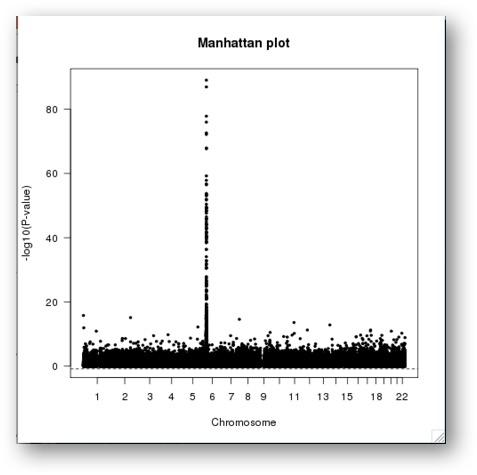
\includegraphics[width=8cm]{figure_1}
    \centering
\end{figure}


% TODO: Add section on plans for this semester


\bibliographystyle{ieeetr}
\bibliography{Thesis}

\end{document}
